\documentclass[border=3pt,tikz]{standalone}
\usepackage{amsmath}
\usetikzlibrary{calc}
\usetikzlibrary{arrows.meta} % for arrow size
\begin{document}

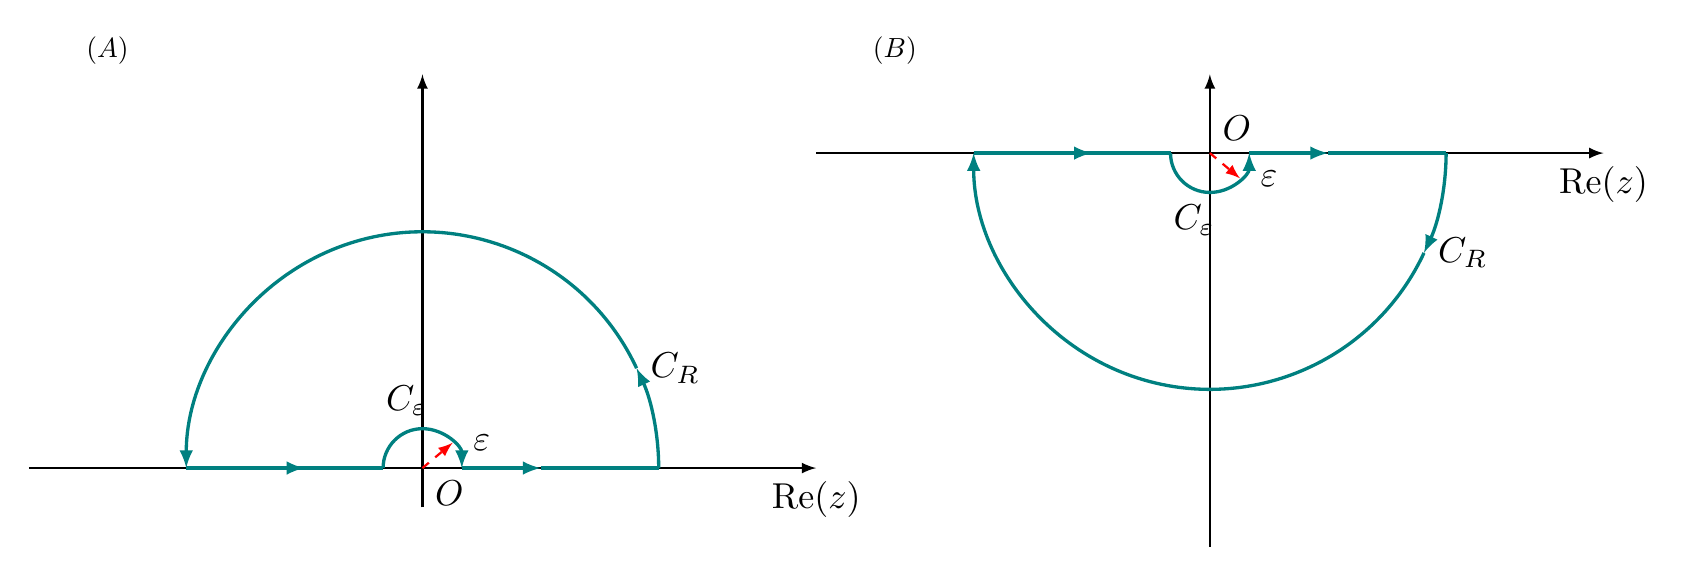
\begin{tikzpicture}[scale=1.0]
    \usetikzlibrary {arrows.meta}
    \usetikzlibrary {calc}
    
    
    \node[above] at (-4, 5) {$(A)$};
    \draw [thick,-latex] (-5, 0) -- (5, 0) node[below, scale=1.3] {Re$(z)$};
    \draw [thick, -latex] (0, -0.5) -- (0, 5);
    
    \draw[teal, very thick, -latex,] (3, 0) arc (0:25:3) node[black,right, scale=1.3] {$C_R$};
    \draw[teal, very thick, -latex,] ({3*cos(25)}, {3*sin(25)}) arc (25:180:3);
    \draw[teal, very thick, -latex] (-3, 0) -- (-1.5, 0);
    \draw[teal, very thick] (-3, 0) -- (-0.5, 0) ;
    \node[above, scale=1.3 ] at (-0.2, 0.5) {$C_\varepsilon$};
    \draw[teal, very thick, -latex] (-0.5, 0) arc (180:0:0.5);
    \draw[teal, very thick, -latex] (0.5, 0) -- (1.5, 0);
    \draw[teal, very thick, ] (1.5, 0) -- (3, 0);
    \draw[red, thick, dashed, -latex] (0, 0) -- ({0.5*cos(40)}, {0.5*sin(40)}) node [black, scale=1.3, right, xshift=2] {$\varepsilon$};
    
    \node[black, scale=1.3, below right] at (0, 0) {$O$};
    
    
    \begin{scope}[shift={(10,4)}]
    \node[above] at (-4, 1) {$(B)$};
    \draw [thick,-latex] (-5, 0) -- (5, 0) node[below, scale=1.3] {Re$(z)$};
    \draw [thick, -latex] (0, -5) -- (0, 1);
    
    \draw[teal, very thick, -latex,] (3, 0) arc (0:-25:3) node[black,right, scale=1.3] {$C_R$};
    \draw[teal, very thick, -latex,] ({3*cos(-25)}, {3*sin(-25)}) arc (-25:-180:3);
    \draw[teal, very thick, -latex] (-3, 0) -- (-1.5, 0);
    \draw[teal, very thick] (-3, 0) -- (-0.5, 0) ;
    \node[below, scale=1.3 ] at (-0.2, -0.5) {$C_\varepsilon$};
    \draw[teal, very thick, -latex] (-0.5, 0) arc (180:360:0.5);
    \draw[teal, very thick, -latex] (0.5, 0) -- (1.5, 0);
    \draw[teal, very thick, ] (1.5, 0) -- (3, 0);
    \draw[red, thick, dashed, -latex] (0, 0) -- ({0.5*cos(-40)}, {0.5*sin(-40)}) node [black, scale=1.3, right, xshift=2] {$\varepsilon$};
    
    \node[black, scale=1.3, above right] at (0, 0) {$O$};
    
    
    \end{scope}
    \end{tikzpicture}
\end{document}